\documentclass[twoside,11pt]{article}

%================================ PREAMBLE ==================================

%--------- Packages -----------
\usepackage{fullpage}
\usepackage{amssymb}
\usepackage{amsmath}
\usepackage{amsthm}
\usepackage{latexsym}
\usepackage{graphicx}
\usepackage{wrapfig}
\usepackage{color}
\usepackage{url}
\usepackage{algorithm,algorithmic}
\usepackage{booktabs}
\usepackage[demo]{graphicx}
\usepackage{caption}
\usepackage{subcaption}
\usepackage{enumitem}


%---------- Spacing ----------
\setlength{\parindent}{0pt}
\setlength{\parskip}{8pt}

%---------Definitions----------
\newcommand{\half}{{\textstyle{\frac{1}{2}}}}
\renewcommand{\>}{{\rightarrow}}
\renewcommand{\hat}{\widehat}
\renewcommand{\tilde}{\widetilde}
\newcommand{\grad}{{\nabla}}
%
\newcommand{\argmax}{\textup{\textrm{argmax}}}
\newcommand{\argmin}{\textup{\textrm{argmin}}}
\newcommand{\argsort}{\textup{\textrm{argsort}}}
\newcommand{\sign}{\textup{\textrm{sign}}}
\newcommand{\poly}{\textup{\textrm{poly}}}
\newcommand{\er}{\textup{\textrm{er}}}
\newcommand{\zo}{\textup{\textrm{0-1}}}
\newcommand{\sq}{\textup{\textrm{sq}}}
%
\newcommand{\1}{{\mathbf 1}}
\newcommand{\0}{{\mathbf 0}}
\newcommand{\I}{{\mathbf I}}
\newcommand{\R}{{\mathbb R}}
\newcommand{\Z}{{\mathbb Z}}
\newcommand{\N}{{\mathbb N}}
\renewcommand{\P}{{\mathbf P}}
\newcommand{\E}{{\mathbf E}}
\newcommand{\Var}{{\mathbf{Var}}}
%
\renewcommand{\a}{{\mathbf a}}
\renewcommand{\b}{{\mathbf b}}
\renewcommand{\c}{{\mathbf c}}
\renewcommand{\d}{{\mathbf d}}
\newcommand{\f}{{\mathbf f}}
\renewcommand{\k}{{\mathbf k}}
\newcommand{\p}{{\mathbf p}}
\newcommand{\q}{{\mathbf q}}
\renewcommand{\u}{{\mathbf u}}
\newcommand{\w}{{\mathbf w}}
\newcommand{\x}{{\mathbf x}}
\newcommand{\y}{{\mathbf y}}
%
\newcommand{\A}{{\mathbf A}}
\newcommand{\bC}{{\mathbf C}}
\newcommand{\C}{{\mathcal C}}
\newcommand{\cD}{{\mathcal D}}
\newcommand{\F}{{\mathcal F}}
\renewcommand{\H}{{\mathcal H}}
\newcommand{\K}{{\mathbf K}}
\renewcommand{\L}{{\mathcal L}}
\newcommand{\bL}{{\mathbf L}}
\newcommand{\cN}{{\mathcal N}}
\newcommand{\W}{{\mathbf W}}
\newcommand{\X}{{\mathcal X}}
\newcommand{\bX}{{\mathbf X}}
\newcommand{\Y}{{\mathcal Y}}
%
\newcommand{\bloss}{{\boldsymbol \ell}}
\newcommand{\blambda}{{\boldsymbol \lambda}}
\newcommand{\bmu}{{\boldsymbol \mu}}
\newcommand{\bnu}{{\boldsymbol \nu}}
\newcommand{\bSigma}{{\boldsymbol \Sigma}}
\newcommand{\seta}{{\boldsymbol \eta}}
\newcommand{\bpsi}{{\boldsymbol \psi}}
\newcommand{\bphi}{{\boldsymbol \phi}}
\newcommand{\bPhi}{{\boldsymbol \Phi}}
\newcommand{\balpha}{{\boldsymbol \alpha}}
\newcommand{\bxi}{{\boldsymbol \xi}}

%=============================== END PREAMBLE ===============================

\begin{document}

%================================ COVER PAGE ================================

\emph{\footnotesize{CIS 620 Fall 2018, Project Report}}

\vspace{12pt}

\begin{center}

%Fill in your project title
\textbf{\Large{Understanding Multiclass Extensions of ROC/AUC and their Relationships}}

\vspace{6pt}

%Fill in author names
Bowen Ke \\ (PennKey: \texttt{bowenke}; Email: \texttt{bowenke@seas.upenn.edu}) \\[4pt]
Hui Lyu \\ (PennKey: \texttt{huilyu}; Email: \texttt{huilyu@seas.upenn.edu}) \\[4pt]
Simeng Sun \\ (PennKey: \texttt{simsun}; Email: \texttt{simsun@seas.upenn.edu}) 

\end{center}

%---

%Add abstract 
\begin{abstract}
There are three multiclass extensions of ROC curve/AUC: pairwise, one-vs-rest and VUS. However, the relationships between them are not well understood. This project has derived comparable mathematical expressions for each of them for theoretical comparison, and also conducted two experiments for empirical analysis of their pros and cons. 
\end{abstract}

\vspace{6pt}

%============================= MAIN DOCUMENT ================================

\section{Introduction}
%HL
% \subsection{Background and Motivation}
A {\em Receiver operating characteristics} (ROC) curve is a 2-dimensional plot where y-axis is the true positive rate (TPR) and x-axis is the false positive rate (FPR). It can be generated by changing the threshold $t$ for a binary classifier $h_t(x) = \text{sign}(f(x) - t)$ where $f$ is a scoring model $f: \mathcal{X}\rightarrow \mathbb{R}$.
The {\em area under the ROC curve} (AUC) is a single number measuring the overall performance of the scoring model. %This area is also equivalent to the probability of a randomly sampled positive example ranking higher than a randomly sampled negative example~. %The ROC curve itself is also used for model selection as a performance metric. In binary cases, the set of potentially optimal classifier lies on the convex hull formed by the points in the ROC space. 
Though AUC for binary problems is well-defined and effective in real cases, the multiclass extensions are not well studied and explained.
% Though binary ROC/AUC is well-defined and effective in real cases, multiclass ROC curves become much more complex. 
% For any classification task of $c (c>2)$ classes, the confusion matrix is of size $c \times c$ with $c(c-1)$ possible errors. 
% Thus, to measure the scoring model performance in the entire space, one can apply different methods. 
There are in general three kinds of ROC/AUC multiclass extensions, each of them has different settings and lacks either statistical explanation or relationship with binary cases. 
Therefore, we aim to understand the relationships among the existing ROC/AUC multiclass extensions and compare them theoretically and empirically.

% \subsection{Contributions}
Our contirbutions are as follows: (1) We unified binary AUC and multiclass AUC extensions using class score density function. (2) We compared multiclass AUC extensions with binary AUC theoretically and analyzed their pros and cons (3) Based on our derived expression, we conducted simulation and explored how class separability and class imbalanace affects each kind of multiclass extensions.

\section{Related work}
%SS
% In this section, we first briefly review \textit{receiver operating characteristic} (ROC) and the area under the ROC curve (AUC) in binary setting, then introduce 3 common multiclass AUC extensions.
\subsection{Preliminaries}
% The ROC curve is a graph in which the true positive rate ($TPR$) is plotted on the Y axis and false positive rate ($FPR$) is plotted on the X axis. %For a binary classification problem with positive and negative classes, we have
% \begin{equation}
%     TPR=\frac{\text{\# of positives correctly classified}}{\text{\# of total positives}}
% \end{equation}
% \begin{equation}
%     FPR=\frac{\text{\# of negatives incorrectly classified}}{\text{\# of total negatives}}
% \end{equation}

The ROC curve can be plotted by varying the threshold given the output of a scoring model $f : \mathcal{X} \rightarrow \mathbb{R}$. Each operating point is a pair of $(FPR, TPR)$ and corresponds to a specific confusion matrix. 
% Several important points to notice. 
% The point $(0,0)$ corresponds to the case where no instance is classified as positive. 
% The point $(1,1)$ is the opposite scenario where every instance is classified as positive. 
% The point $(0,1)$ implies perfect performance. The line $y=x$ represent a random classifier; any point below the line $y=x$ can be project to the upper left half space, therefore every point must be in the upper left part. 
The area under the curve is a  scalar performance measure for evaluating classifiers. Closely related to the Gini Coefficient, it is the probability a randomly chosen positive instance having higher rank than a randomly chosen negative instance~\cite{Fawcett2006}.

\begin{figure}[h]
    \centering
    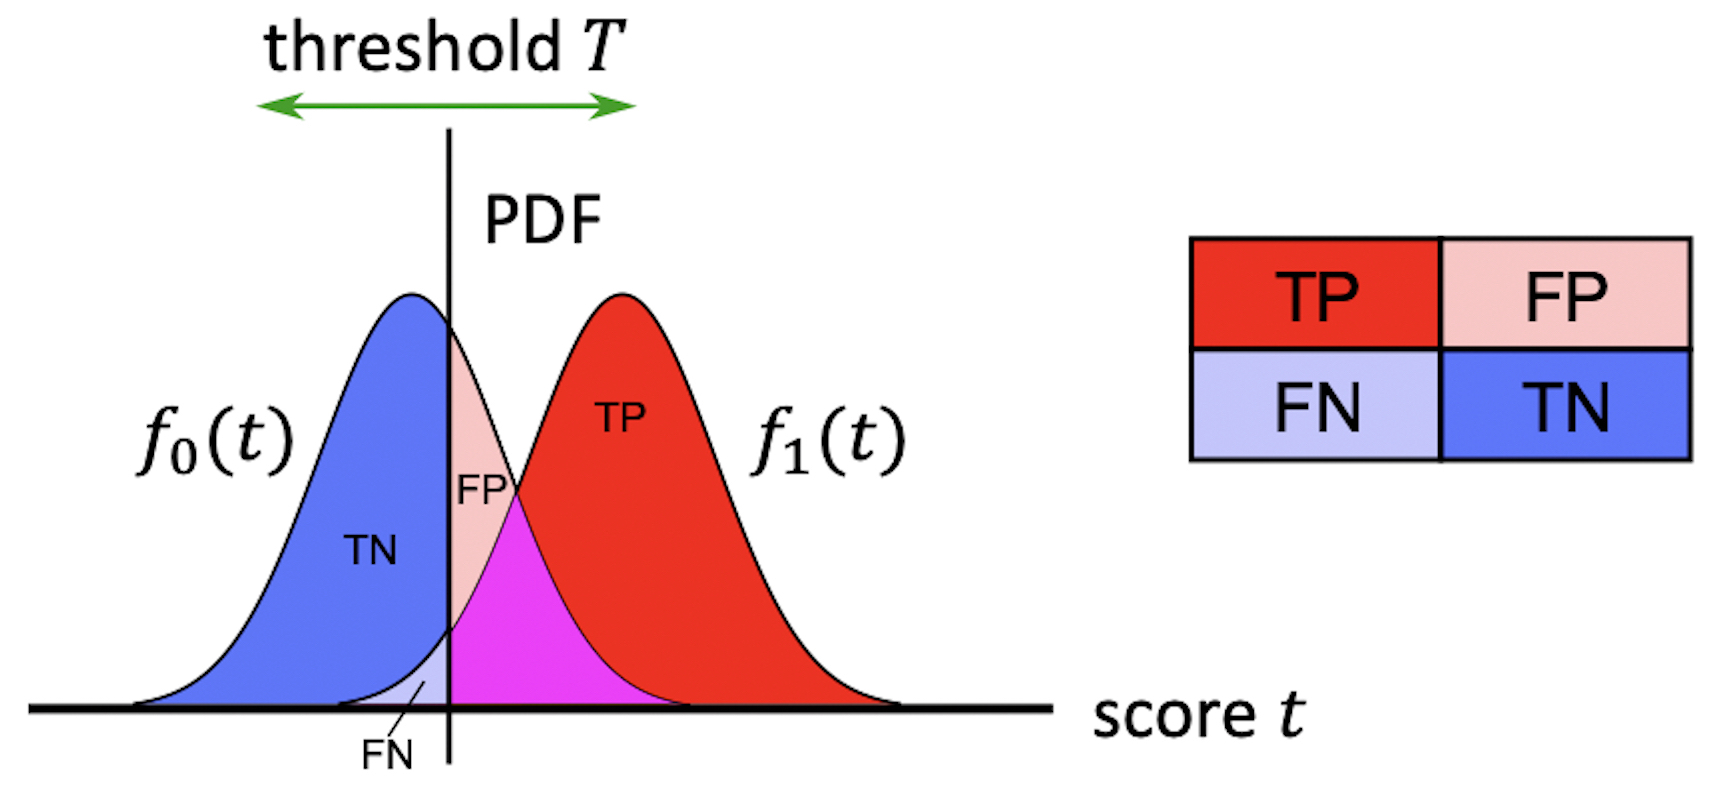
\includegraphics[width=0.4\textwidth]{./pic/binary_ROC.png}
    \caption{Class score density for binary problem. $f_1(t)$ is the score distribution for positives and $f_0(t)$ is the score distribution for negatives}
    \label{fig:binary_roc}
\end{figure}

Both true positive rate and false positive rate can be related to threshold in a form of integral $TPR=\int_{T}^{\infty}f_1(t)dt$, $FPR = \int_{T}^{\infty}f_0(t)dt$,
% \begin{equation} \label{eq_TPR}
%     TPR = \int_{T}^{\infty}f_1(t)dt
% \end{equation}
% \begin{equation} \label{eq_FPR}
%     FPR = \int_{T}^{\infty}f_0(t)dt
% \end{equation}
where the score of positives follows the probability density function $f_1(\cdot)$, that of negatives follows $f_0(\cdot)$. The densities are jointly decided by the classifier and the data set. There is previous work estimating such distribution using Gaussian Mixture Model  \cite{gmm}. A more generic depiction is shown in Figure \ref{fig:binary_roc}\footnote{Image from wikipedia: https://upload.wikimedia.org/wikipedia/commons/thumb/4/4f/ROC\_curves.svg/600px-ROC\_curves.svg.png}. True positive rate is therefore the area under $f_1(t)$ when $t$ is greater than certain threshold $T$. $T$ tending to infinity corresponds to the point $(0,0)$ in ROC space. %In section 4.1, we will show how to represent AUC using the threshold and class score distributions. 

\subsection{Multiclass AUC}

There are in general 3 kinds of multiclass AUC extensions, two of which are approximations to the real exact number that characterizes the performance of a multiclass classifier. 

\subsubsection{Pairwise}\label{sec:pairwise-intro}
One approximation approach is the Pairwise AUC~\cite{Hand2001}. It measures what the authors called ``separability'' of each pair of classes and originates directly from the statistical meaning of bianry AUC. Suppose there are total $c$ classes, for each of the ${c \choose 2}$ pair of classes, they use $A(c_i, c_j)$ as a measure of the separability for class $c_i$ and $c_j$. Pairwise AUC is the unweighted average over  $A(c_i,c_j)$ of each pair of classes.\\
\begin{equation}\label{eq:pairwise-AUC}
    \text{AUC}_{\text{pairwise}} = \frac{2}{c(c-1)}\sum\limits_{c_i<c_j}A(c_i,c_j)
\end{equation}
The separability of each pair is an average of $A(c_i|c_j)$ and $A(c_j|c_i)$, where $A(c_i|c_j)$ is the probability that a randomly drawn instance from class $c_i$ has a higher estimated probability of belong to class $c_i$ than a randomly drawn instance from class $c_j$.
% Applying to scoring model, it is equivalent to say it is the probability of randomly drawn instance from class $j$ has lower score for class $i$ than a randomly drawn instance from class $i$.
% This approach involves computing ${c \choose 2}$ AUCs, given each AUC runs in time $O(n\log n)$, the running time for computing pairwise AUC is thus $O(c^2n\log n)$.

\subsubsection{One-vs-Rest}\label{sec:1-vs-rest}
Another kind of multiclass AUC extension adopts an one-vs-rest strategy \cite{Provost2003}. This kind of AUC is a weighted average of $c$ AUCs. $\text{AUC}(c_i)$ is the area under a ROC curve which is plotted by viewing only $c_i$ as positive and the union of the rest $c-1$ classes as negative. $p(c_i)$ is the prevalence of class $c_i$ among total $m$ instances.
\begin{equation}\label{eq:1-vs-rest}
    \text{AUC}_{\text{1-vs-rest}} = \sum\limits_{i=1}^c \text{AUC}(c_i) p(c_i)
\end{equation}
\begin{equation}
    p(c_i) = \frac{\sum\limits_{j=1}^m\mathbb{I}(y_j=c_j)}{m}
\end{equation}
% This approach involves computing $c$ AUCs, the running time is $O(cn\log n)$. 

\subsubsection{Volume under hyper-surface}
The most exact generalization of multiclass AUC is the volume under hyper-surface (VUS). Pairwise and one-vs-rest are approximations to the exact VUS. 
% It has been shown the optimal multiclass classifier lies on a $c(c-1)$-dimensional polytope \cite{Srinivasan99}. 
% There are also papers showing the off-diagonal entries of a confusion matrix corresponds to an operating point in the $c(c-1)$-dimensional ROC space \cite{VUS}. 
VUS is a direct extension of binary AUC where we change the y-axis $TPR$ to false negative rate ($FNR$). The optimal classifier for this kind of ROC variant has the minimum possible area under the curve. Consider all off-diagonal entries in a confusion matrix, it maps to an operating point in $c(c-1)$-dimensional space. Extending directly from the binary ROC variant, the volume under the hyper-surface formed by varying a set of thresholds is expected to be the minimum for optimal classifiers. When there are 3 classes, it becomes immediately difficult to analyze and visualize since the surface is in 6-dimensional space. This is the reason why people reduce the true extension to binary cases where good interpretability and visualization preserve. 

Besides, there is another kind of VUS which is an approximation to the real VUS where only the diagonal entries of a confusion matrix are considered and therefore corresponds to a point in a $c$-dimensional space \cite{VUS-2}. The real VUS is computed by transforming to a constraint satisfaction problem. The maximum and minimum VUS can be computed by enforcing constraint subject to normalized confusion matrix. However, the authors didn't provide any analytical expression for the exact VUS.

\section{Problem settings and notations}
%SS
We consider general multiclass classification problems. We do not require the classes to satisfy certain order. 
The number of classes is denoted by $c$.
We consider socring model where there are total $c$ scoring functions $s_1, \dots, s_c$, each instance gets a $c$-dimensional score vector $S(\textbf{x}) = (s_1(\textbf{x}), \dots, s_c(\textbf{x}))^{\top}$. 
We define $f_{ij}(\cdot)$ to be probability density function of the $i^{\text{th}}$ entry of $S(\textbf{x})$ for every instance $\textbf{x}$ belonging to class $j$.
% \begin{itemize}
%     \item We consider general multiclass classification problems. We do not require the classes to satisfy certain order. 
%     \item The number of classes is denoted by $c$.
%     \item We consider socring model where there are total $c$ scoring functions $s_1, \dots, s_c$, each instance gets a $c$-dimensional score vector $S(\textbf{x}) = (s_1(\textbf{x}), \dots, s_c(\textbf{x}))^{\top}$ and is classified to $\hat{y} = \argmax_{i}s_i(\textbf{x})$
%     \item We define $f_{ij}(\cdot)$ to be probability density function of the $i^{\text{th}}$ entry of $S(\textbf{x})$ for every instance $\textbf{x}$ belonging to class $j$.
% \end{itemize}

\section{Theoretical analysis}
In this section, we rederive the integral form of binary AUC and show how it can be unified with multiclass AUC extensions using the score density function $f_{ij}(\cdot)$ and the thresholds $T_{ij}$ (introduced later). %firstly rederive the mathematical expression of binary AUC in terms of threshold. Then we derive multiclass AUC expressions for pairwise, one-vs-rest and VUS approaches respectively in terms of $f_{ij}(\cdot)$ (PDF) and threshold, to make them comparable.
% express binary AUC and multicalss AUC in terms of threshold and score distribution

\subsection{Binary AUC}
%SS
According to the integral form of TPR and FPR and the geometry meaning of AUC, we have the following expression for binary AUC:
\begin{align}\label{eq_binary_AUC}
    \text{AUC}_{\text{binary}} &= \int_{\infty}^{-\infty}TPR(T)FPR'(T)dT\\
    &= \int_{\infty}^{-\infty}(\int_{T}^{\infty}f_1(T')dT')(-f_0(T))dT\\
    &= \int_{-\infty}^{\infty}\int_{-\infty}^{\infty}\mathbb{I}(T'>T)f_1(T')f_0(T)dT'dT
\end{align}


The integration in equation \ref{eq_binary_AUC} is from infinity to negative infinity since we integrate $FPR$ from 0 to 1, which is equivalent to varying threshold from $\infty$ to $-\infty$. Intuitively, it can be interpreted as putting two thresholds on the score distribution, one for each $f_i(\cdot)$ and both vary from $-\infty$ to $\infty$. Then AUC is the area where the threshold for $f_1(t)$ is larger than that for $f_0(t)$. The upper left area above the ROC curve is thus characterized by the indicator function $\mathbb{I}(T' \leq T)$.

\subsection{Pariwise}
%HL
  Pairwise AUC, which has been introduced in Section~\ref{sec:pairwise-intro} is the unweighted ``sperability'' of each pair of classes. The separability between class $i$ and class $j$ is the average of $A(i|j)$ and $A(j|i)$. Extending their explanation for CPE model, in our setting, $A(i|j)$ is the probability that the $i^{\text{th}}$ score of a random instance from class $i$ is greater than the $i^{\text{th}}$ score of an instance randomly drawn from class $j$, $\forall j \neq i$. Notice that $\text{AUC}_{\text{binary}} = A(1|0)$, which builds a connection between binary AUC and pairwise multiclass AUC. Figure \ref{fig:pairwise} shows 6 possible pairs for a 3-class classification problem. $A(1|3)$ represents the case in which we select class 1 as positive and class 3 as negative.  Recall we require that a classifier associates each instance with a $c$-dimensional score vector $S(\textbf{x}) = (s_1(\textbf{x}), \dots, s_c(\textbf{x}))^{\top}$. To transform their notion of ``separability'' into our setting, we have:
\begin{equation}
    A(i,j) = \frac{1}{2}(A(i|j) + A(j|i)) = \frac{1}{2}\Big( P\big(s_i(\mathbf{x}^{(i)}) > s_i(\mathbf{x}^{(j)})\big) + P\big(s_j(\mathbf{x}^{(j)}) > s_j(\mathbf{x}^{(i)})\big) \Big)
\end{equation}
where $\mathbf{x}^{(i)}$ represents an instance from class $i$, $s_i(\mathbf{x}^{(i)})$ denotes the $i^{\text{th}}$ score associated with that instance.
% The notation $\mathbf{x}^{(i)}$ represents the feature vector of an instance from class $i$, and $s_i(\mathbf{x}^{(i)})$ denotes the $i^{\text{th}}$ score associated with that instance. $A(i|j)$ is the probability that the $i^{\text{th}}$ score of an instance from class $i$ is greater than the $i^{\text{th}}$ score of any other instance from class $j$ ($i < j$). Vice versa for $A(j|i)$. Notice that $\text{AUC}_{\text{binary}} = A(1|0)$, which builds a connection between binary AUC and pairwise multiclass AUC. 

% For example, Figure~\ref{fig:pairwise} 
% \begin{figure}[h]
%     \centering
%     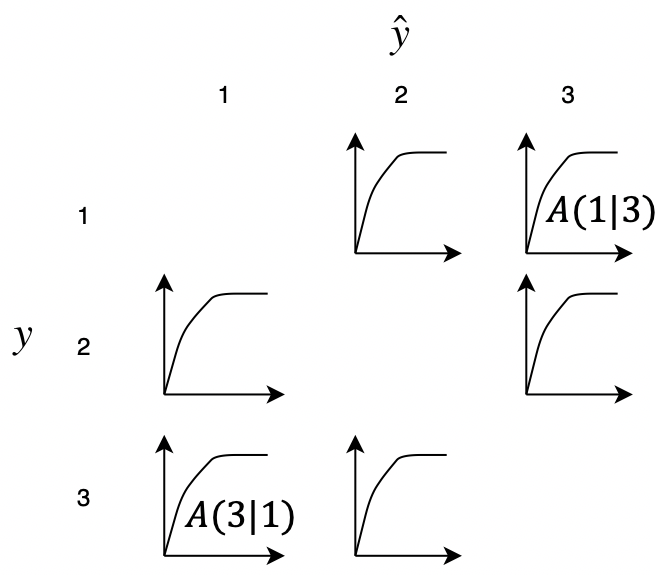
\includegraphics[width=0.34\textwidth]{pic/pairwise.png}
%     \caption{Multiclass pairwise choices for 3-class classification}
%     \label{fig:pairwise}
% \end{figure}

\begin{figure}
\centering
\begin{minipage}{.5\textwidth}
  \centering
  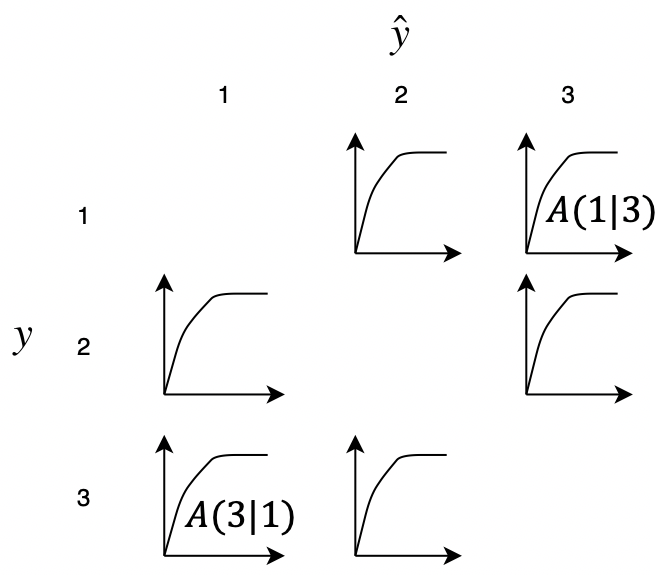
\includegraphics[width=.6\linewidth]{pic/pairwise.png}
  \captionof{figure}{Multiclass pairwise choices}
  \label{fig:pairwise}
\end{minipage}%
\begin{minipage}{.5\textwidth}
  \centering
  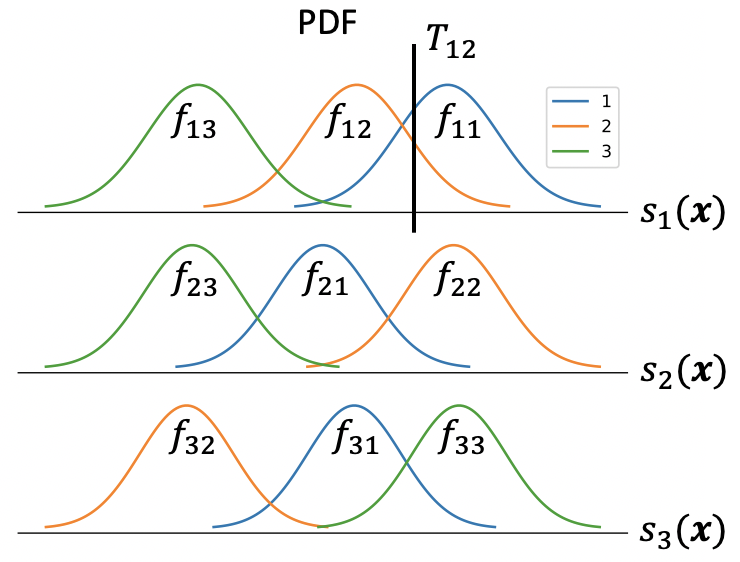
\includegraphics[width=.6\linewidth]{pic/PDF.png}
  \captionof{figure}{One possible $f_{ij}(\cdot)$ distribution for 3-class classification}
  \label{fig:PDF}
\end{minipage}
\end{figure}

Further, we describe the probabilities with $f_{ij}$ and thresholds $T_{ij}$:
\begin{align}
    P\big(s_i(\mathbf{x}^{(i)}) > s_i(\mathbf{x}^{(j)})\big) &= \int_{−\infty}^{\infty}\int_{−\infty}^{\infty}\mathbb{I}(T_{ij}>T_{ij}')f_{ii}(T_{ij}')f_{ij}(T_{ij})dT_{ij}'dT_{ij} \\
    P\big(s_j(\mathbf{x}^{(j)}) > s_j(\mathbf{x}^{(i)})\big) &= \int_{−\infty}^{\infty}\int_{−\infty}^{\infty}\mathbb{I}(T_{ji}>T_{ji}')f_{jj}(T_{ji}')f_{ji}(T_{ji})dT_{ji}'dT_{ji}
\end{align}
where $T_{ij}$ denotes the threshold on the $i^{\text{th}}$ score axis for distinguishing instances belonging to class $i$ and instances belonging to class $j$. Figure~\ref{fig:PDF} generically demonstrates one possible distribution of $f_{ij}(\cdot)$ for a 3-class classification problem.
% \begin{figure}[h]
%     \centering
%     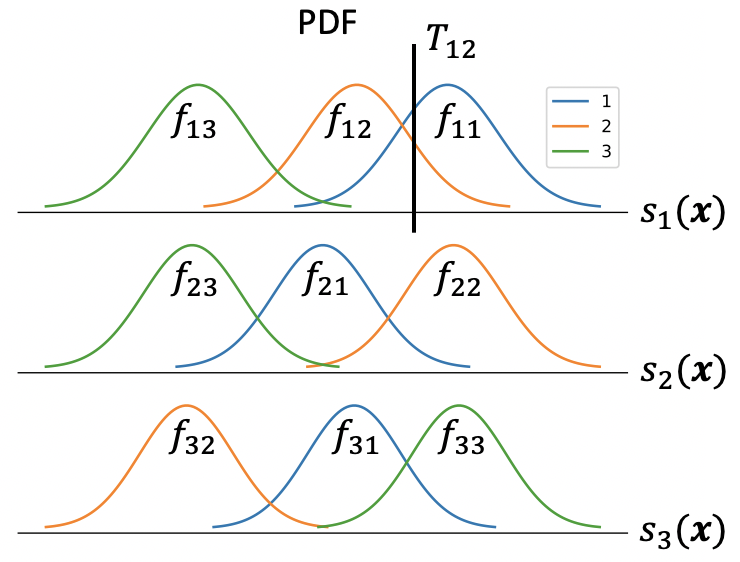
\includegraphics[width=0.35\textwidth]{pic/PDF.png}
%     \caption{One possible $f_{ij}(\cdot)$ distribution for 3-class classification}
%     \label{fig:PDF}
% \end{figure}

Based on Equation~\ref{eq:pairwise-AUC}, we derive pairwise AUC using $f_{ij}(\cdot)$ and $T_{ij}$:
\begin{align}
    \text{AUC}_{\text{pairwise}} &= \frac{2}{c(c-1)}\sum\limits_{i<j}A(i,j) \\
    &= \frac{2}{c(c-1)}\sum\limits_{i<j} \Big[\frac{1}{2}\Big( P\big(s_i(\mathbf{x}^{(i)}) > s_i(\mathbf{x}^{(j)})\big) + P\big(s_j(\mathbf{x}^{(j)}) > s_j(\mathbf{x}^{(i)})\big) \Big)\Big] \\
    &= \frac{2}{c(c-1)}\sum\limits_{i<j}\frac{1}{2}\Big(\int_{−\infty}^{\infty}\int_{−\infty}^{\infty}\mathbb{I}(T_{ij}>T_{ij}')f_{ii}(T_{ij}')f_{ij}(T_{ij})dT_{ij}'dT_{ij} \\& +\int_{−\infty}^{\infty}\int_{−\infty}^{\infty}\mathbb{I}(T_{ji}>T_{ji}')f_{jj}(T_{ji}')f_{ji}(T_{ji})dT_{ji}'dT_{ji}\Big)
\end{align}
To further understand the meaning of pairwise multiclass AUC, we find that
\begin{equation}
    \text{AUC}_{\text{pairwise}} = \frac{1}{c(c-1)} \sum\limits_{i \neq j} P\big(s_i(\mathbf{x}^{(i)}) > s_i(\mathbf{x}^{(j)})\big) %P_i (X_i > X_j)
\end{equation}
% where $P\big(s_i(\mathbf{x}^{(i)}) > s_i(\mathbf{x}^{(j)})\big)$ denotes the probability that the $i^{\text{th}}$ score of a randomly drawn instance from class $i$ is greater than that of a randomly drawn instance from class $j$. %any instance from class $i$ is greater than the $i^{\text{th}}$ score of any other instance from class $j$ ($j \neq i$). 
It is an arithmetic mean (unweighted) of all the $c(c-1)$ positive-negative pairs of binary AUC and thus should be insensitive to class imbalance.

\subsection{One-vs-Rest}
%HL
Based on the discussion in Section~\ref{sec:1-vs-rest}, we derive the expression for $\text{AUC}(c_i)$ within our setting.
\begin{equation}
    \text{AUC}(c_i) = \int_{−\infty}^{\infty}\int_{−\infty}^{\infty}\mathbb{I}(T'>T)f_{ii}(T')\frac{[\sum\limits_{j\neq i}f_{ij}(T)]}{c-1}dT'dT = \frac{1}{c-1} \sum\limits_{j \neq i} P\big(s_i(\mathbf{x}^{(i)}) > s_i(\mathbf{x}^{(j)})\big)
\end{equation}
where $\frac{[\sum\limits_{j\neq i}f_{ij}(T)]}{c-1}$ represents the distribution of the rest $c-1$ classes. The summation over $f_{ij}(\cdot)$ is normalized by $c-1$ to maintain the property of a PDF.
% $\frac{[\sum\limits_{j\neq i}f_{ij}(T)]}{c-1}$ as the term implying a summation over the PDF of the rest $c-1$ classes and normalized by $c-1$ to preserve the as a PDF. 
% The summation of probabilities is for all $j$, $\forall j \neq i$.
For one-vs-rest method, one can choose any class as positive, and the rest $c-1$ classes as negative, which implies $c$ pairs of binary AUC in total. Finally, we get
\begin{align}
    \text{AUC}_{\text{1-vs-rest}} &= \sum\limits_{i=1}^c \text{AUC}(c_i) p(c_i) \\
    &= \sum\limits_{i=1}^c p(c_i) \int_{−\infty}^{\infty}\int_{−\infty}^{\infty}\mathbb{I}(T'>T)f_{ii}(T')\frac{[\sum\limits_{j\neq i}f_{ij}(T)]}{c-1}dT'dT \\
    &= \sum\limits_{i=1}^c p(c_i) \frac{1}{c-1} \sum\limits_{j \neq i} P\big(s_i(\mathbf{x}^{(i)}) > s_i(\mathbf{x}^{(j)})\big)
\end{align}
where $p(c_i) = \frac{\sum\limits_{i=1}^m\mathbb{I}(y_i=c_i)}{m}$. Therefore, 1-vs-rest multiclass AUC is a weighted arithmetic mean of all the $c$ pairs of binary AUC.

\subsection{Volume Under Hyper-Surface}
%SS
In this section, we present a tentative form for VUS within our setting. For binary AUC, we can transform the ROC curve by changing $y$-axis $FNR$ and the minimum area is expected for optimal classifiers. 
Naturally extending this to multiclass, we look into the tuples of all off-diagonal entries of a confusion matrix. 
% We will show our derivation first on a simple 3-class problems, then generalize the result to problems with any number of classes. 
Given confusion matrix in table \ref{tab:confusion_matrix}, we can transform the tuple $(b,c,d,f,g,h)$ to a point in ROC space $(\frac{b}{m_1-c}, \frac{c}{m_1-b}, \frac{d}{m_2-f}, \frac{f}{m_2-d}, \frac{g}{m_3-h}, \frac{h}{m_3-g})$ where $m_1$, $m_2$, $m_3$ is the number of instances belonging to class $1,2, 3$ respectively. We will denote each dimension of an operating point in ROC space as false rate $FR(\cdot)$ .
\begin{table}[h]
    \centering
    \begin{tabular}{ccccc}
        
       & & \multicolumn{3}{c}{$\hat{y}$} \\ \cline{2-5}
       &  &  1 & 2 & 3 \\ \cline{2-5}
       & 1 &  a & b & c \\
      $y$ & 2 &  d & e & f \\
       & 3 &  g & h & i \\ \cline{2-5}
        
    \end{tabular}
    \caption{A confusion matrix for 3-class multiclass classification.}
    \label{tab:confusion_matrix}
\end{table}

Inspired by the form of binary AUC which we showed in section 4.1 that the function $\mathbb{I}(T'>T)$ indicates the area in 2D space that should be under the ROC curve. %It can also be further simplified to the form
% \begin{equation}
%     \text{AUC}_{\text{binary}} = \int_{FPR(T)=0}^{FPR(T)=1}\int_{TPR(T')=0}^{TPR(T')=1}\mathbb{I}(T'>T)d(TPR(T'))d(FPR(T))
% \end{equation}
Generalizing to VUS, the volume has a similar form where a function indicating which region is below the surface and integrate this function over each axis. However, instead of integrating over a single threshold as what we did for binary case, each axis of the multiclass ROC space should, instead, be a hyper space defined by multiple thresholds. Specifically, the dimension corresponding to $\frac{b}{m_1-c}$ has the form 
\begin{align*}
    D_{21}(\textbf{T}^{(21)}) = & \int_{FR(T_{13})=0}^{FR(T_{13})=1}\int_{FR(T_{12})=0}^{FR(T_{12})=1}\int_{FR(T_{31})=0}^{FR(T_{31})=1}\int_{FR(T_{21})=0}^{FR(T_{21})=1}\mathbb{I}(g(T_{21}, T_{31}, T_{12}, T_{13}))\\
    & dFR(T_{21})dFR(T_{31})dFR(T_{12})dFR(T_{13})
\end{align*}
Where $\textbf{T}^{(21)}$ is a set of thresholds $\{T_{21}, T_{31}, T_{12}, T_{13}\}$, $g(T_{21}, T_{31}, T_{21}, T_{13})$ inside the indicator function characterizes the space under the ROC surface for dimension $D_{21}$. Unlike in binary space where only one threshold defines each axis, a set of $2c-2$ thresholds jointly define one axis for multiclass ROC space. The thresholds that defines the entry $b$ in the confusion matrix should be $T_{21}, T_{31}, T_{12}, T_{13}$ which has the same meaning as we defined above. Generalizing to $c$ class problems, the set of thresholds for the entry where $y=i$ and $\hat{y}=j$ is the $2c-2$ thresholds that differentiates class $i$ from the rest of classes and class $j$ from the rest of classes. To generalize to problems of $c$ classes, each dimension can have the form
\begin{equation}
    D_{ij}(\textbf{T}^{(ij)}) = \underbrace{\int\dots\int_{FR_{ik}(T_{ik}) = 0}^{FR_{ik}(T_{ik})=1}}_{2c-2}
\underbrace{\mathbb{I}\big(g(\{T_{ik}, T_{kj} \mid \forall k\in \mathcal{C}, i \neq k, j \neq k\})\big)}_{\mathbb{I}_{ij}(\textbf{T}^{(ij)})}
\underbrace{\prod_{i\neq k, j \neq k} d FR_{ik}(T_{ik})d FR_{kj}(T_{kj})}_{d\textbf{F}_{ij}}
\end{equation}
Using $\mathbb{I}_{ij}(\textbf{T}^{(ij)})$ to simplify the indicator function and $d\textbf{F}_{ij}$ to express the object being integrated, we derive the expression for exact VUS,
\begin{equation}
    \text{AUC}_{\text{VUS}} = \underbrace{\int\ldots\int}_{2c-2} \mathbb{I}_{12}(\textbf{T}^{(12)})\underbrace{\int\ldots\int}_{2c-2} \mathbb{I}_{13}(\textbf{T}^{(13)})\dots\underbrace{\int\ldots\int}_{2c-2} \mathbb{I}_{c(c-1)}(\textbf{T}^{(c(c-1))})d\textbf{F}_{c(c-1)}\dots d\textbf{F}_{13}d\textbf{F}_{12}
\end{equation}

\subsection{Comparison}
%HL
We summarize the comparison result of the three AUC multiclass extensions as a table shown in Table~\ref{tab:compare}.

\begin{table}[h]
\centering
\scalebox{0.9}{
\begin{tabular}{p{2.2cm}|p{4.5cm}|p{4.5cm}|p{4.5cm}}
\hline
Method & Multiclass AUC & Pros & Cons\\\hline
Pairwise & $\frac{1}{c(c-1)} \sum\limits_{i \neq j} P\big(s_i(\mathbf{x}^{(i)}) > s_i(\mathbf{x}^{(j)})\big)$, $O(c^2n\log n)$ & insensitive to class distribution and error costs & hard to visualize the computed surface, not scalable\\ \hline
One-vs-Rest & $\sum\limits_{i=1}^c p(c_i) \frac{1}{c-1} \sum\limits_{j \neq i} P\big(s_i(\mathbf{x}^{(i)}) > s_i(\mathbf{x}^{(j)})\big)$, $O(cn\log n)$ & curves can be easily generated and visualized & sensitive to class distributions and error costs\\ \hline
% VUS & $\prod\limits_{i<j}\frac{P_i(X_i > X_j) + P_j(X_j > X_i)}{2}$ (guess) & ideal multiclass extension as a polytope & multiple definitions, not scalable, hard to visualize\\
VUS & (haven't figured out due to the presence of $g(\textbf{T})$) & ideal multiclass extension, exact number to measure the performance & multiple definitions, not scalable, hard to visualize\\

\hline
\end{tabular}
}
\caption{\label{tab:compare}Comparison of three AUC multiclass extensions.}
\end{table}

\section{Experiments}
We empirically explore how \textit{class separability} and \textit{class imbalance} affect the multiclass AUC extensions. For \textit{class separability}, we compute both pairwise and one-vs-rest AUCs under different separability settings. 
%We consider $4$ scenarios for any class and there are a total of $20$ scenarios for $3$-class classification problems, as shown in \ref{fig:separability}. 
For \textit{class imbalance}, we are interested in how one-vs-rest multiclass AUC reacts under different class prior probability assumptions.% to validate our findings in Table~\ref{tab:compare}. 

\subsection{Class separability}
%SS HL
\subsubsection{Setup}
Although our experiments are set to 3-class settings, it can be easily generated to problems with more classes. For 3-class problem, we have 9 PDF $f_{ij}(\cdot), \forall i,j\in\{1,2,3\}$, assuming each of which follows normal distribution with unit variance.
% Note that we assume unit variance over all PDFs and 
Only the means are varied since variance also affects separability~\cite{Hand2001}. We consider $4$ cases of different class separability for 3-class problem ([o],[a],[b],[c] as explained in Figure \ref{fig:separability}(a)). 
%For each score axis and 
%\textbf{a)} distributions are very close; \textbf{b)} distributions are very a far; \textbf{c), d)} one of the distributions is very a far while the rest two are very close. 
% separability case, we assign a combination of $\mu$ to simulate, as is shown in Figure~\ref{fig:separability}(a). 
There are 3 score axes for 3-class classification, each of which corresponds to any separability case. 
%PDF can be separable on 0,1,2 or 3 axes. 
Hence, there are 20 scenarios in total as demonstrated in Figure~\ref{fig:separability}(b). We assume 3 classes are evenly distributed ($ p(c_i)=\frac{1}{3}, \forall i$ for one-vs-rest AUC).

\begin{figure}[htb]
    \centering
    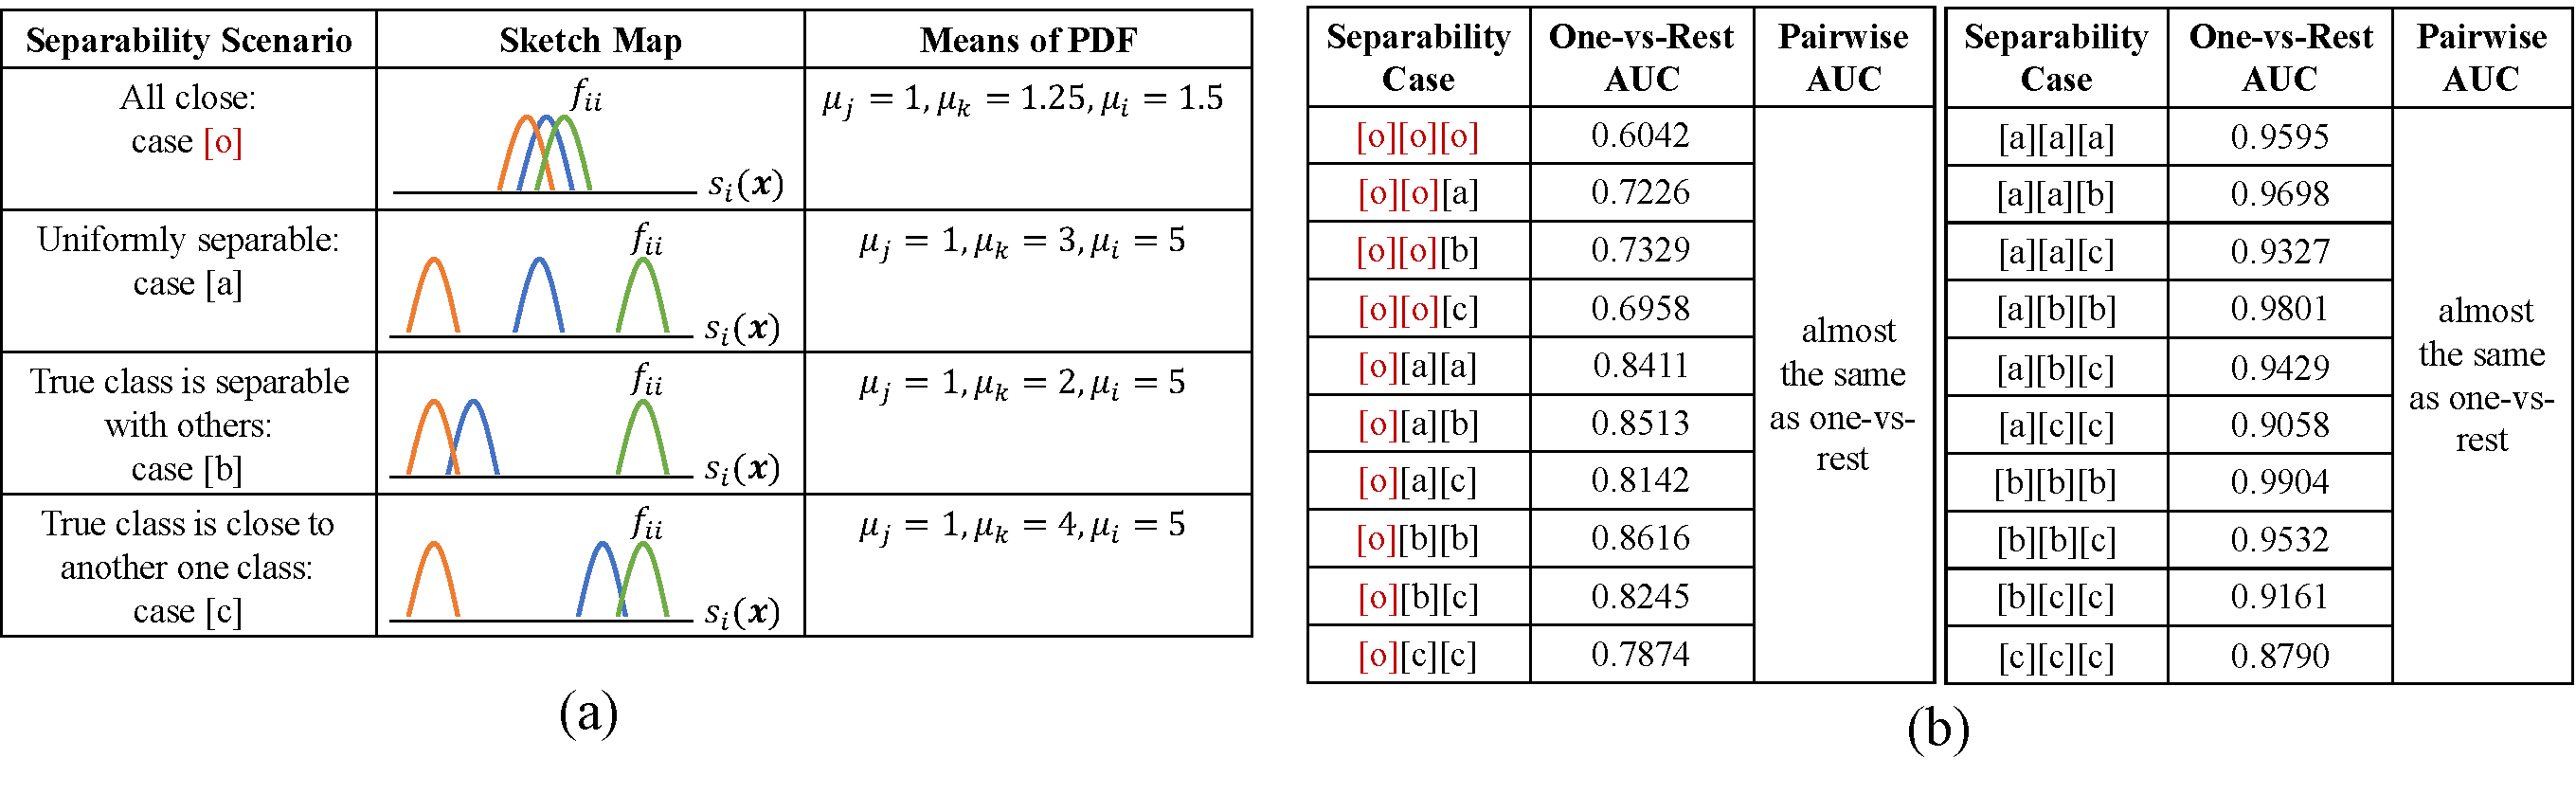
\includegraphics[scale=0.36]{pic/separable.pdf}
    \caption{(a) Separability scenarios for 3 classes; (b) AUC for each separability case. (Pairwise AUC is omitted as it is almost identical to One-vs-Rest AUC, with an average L1 distance of $2\times 10^{-7}$.) }
    \label{fig:separability}
\end{figure}

\subsubsection{Results and discussion}
Figure~\ref{fig:separability}(b) shows that when data is balanced among classes, one-vs-rest and pairwise methods produce almost the same AUC values under different separability cases. %%
We also find that, in general, AUC value decreases when more
% PDFs are close to each other
classes are close to each other
(more case [o]). For separable cases, AUCs in case [b] are slightly higher than AUCs in case [a]. AUCs in case [c] are lower than AUCs in case [a]. We have prior knowledge that case [b], case [a], case [c] and case [o] have a decreasing easiness in terms of separability and that easier separable cases should have higher AUC values. The experimental findings meet our expectation, which also implies that both one-vs-rest and pairwise AUC values are reasonable as a good metric.

\subsection{Class imbalance for one-vs-rest}
% For binary ROC curves, they are insensitive to changes in class distribution. However, based on Equation~\ref{eq:1-vs-rest}, we know that one-vs-rest multiclass ROC is sensitive to class imbalance. 
In this section, we explore how class imbalance affects the one-vs-rest AUC.

\subsubsection{Setup}
Considering 3-class classification, for some PDF $f_{ij}$'s, we vary $p(c_i)$ for one-vs-rest method. We choose entropy as the measurement of class imbalance. Higher entropy means lower extent of class imbalance. Without loss of generality, we fix $p(c_1)=\frac{1}{3}$, and vary $p(c_2)$ and $p(c_3)$ to achieve different entropy values. The entropy is calculated as $H=-\sum_{i=1}^3 p(c_i)\log_3 p(c_i)$.
Although pairwise AUC is unchanged under different class distributions, we compute its value as reference.

We consider two separability cases in this experiment. One situation (Situation A) is where the 3 PDFs on each score axis obey the same distributions, and the other situation (Situation B) is when they are different. We choose one representative distribution for each situation:
\begin{itemize}
\item Situation A: 
$\forall i,j \ f_{ij} \sim N(\mu_{ij},1)$. $\mu_{11}=5,\mu_{12}=3,\mu_{13}=1, \mu_{21}=1,\mu_{22}=5,\mu_{23}=3, \mu_{31}=1,\mu_{32}=3,\mu_{33}=5$
\item Situation B: 
$\forall i,j \ f_{ij} \sim N(\mu_{ij},1)$. $\mu_{11}=1.5, \mu_{12}=1.25, \mu_{13}=1, \mu_{21}=1, \mu_{22}=5, \mu_{23}=3, \mu_{31}=1, \mu_{32}=4, \mu_{33}=5$
\end{itemize}


\subsubsection{Results and discussion}

\begin{figure*}[t!]
    \centering
    \begin{subfigure}[b]{0.5\textwidth}
        \centering
        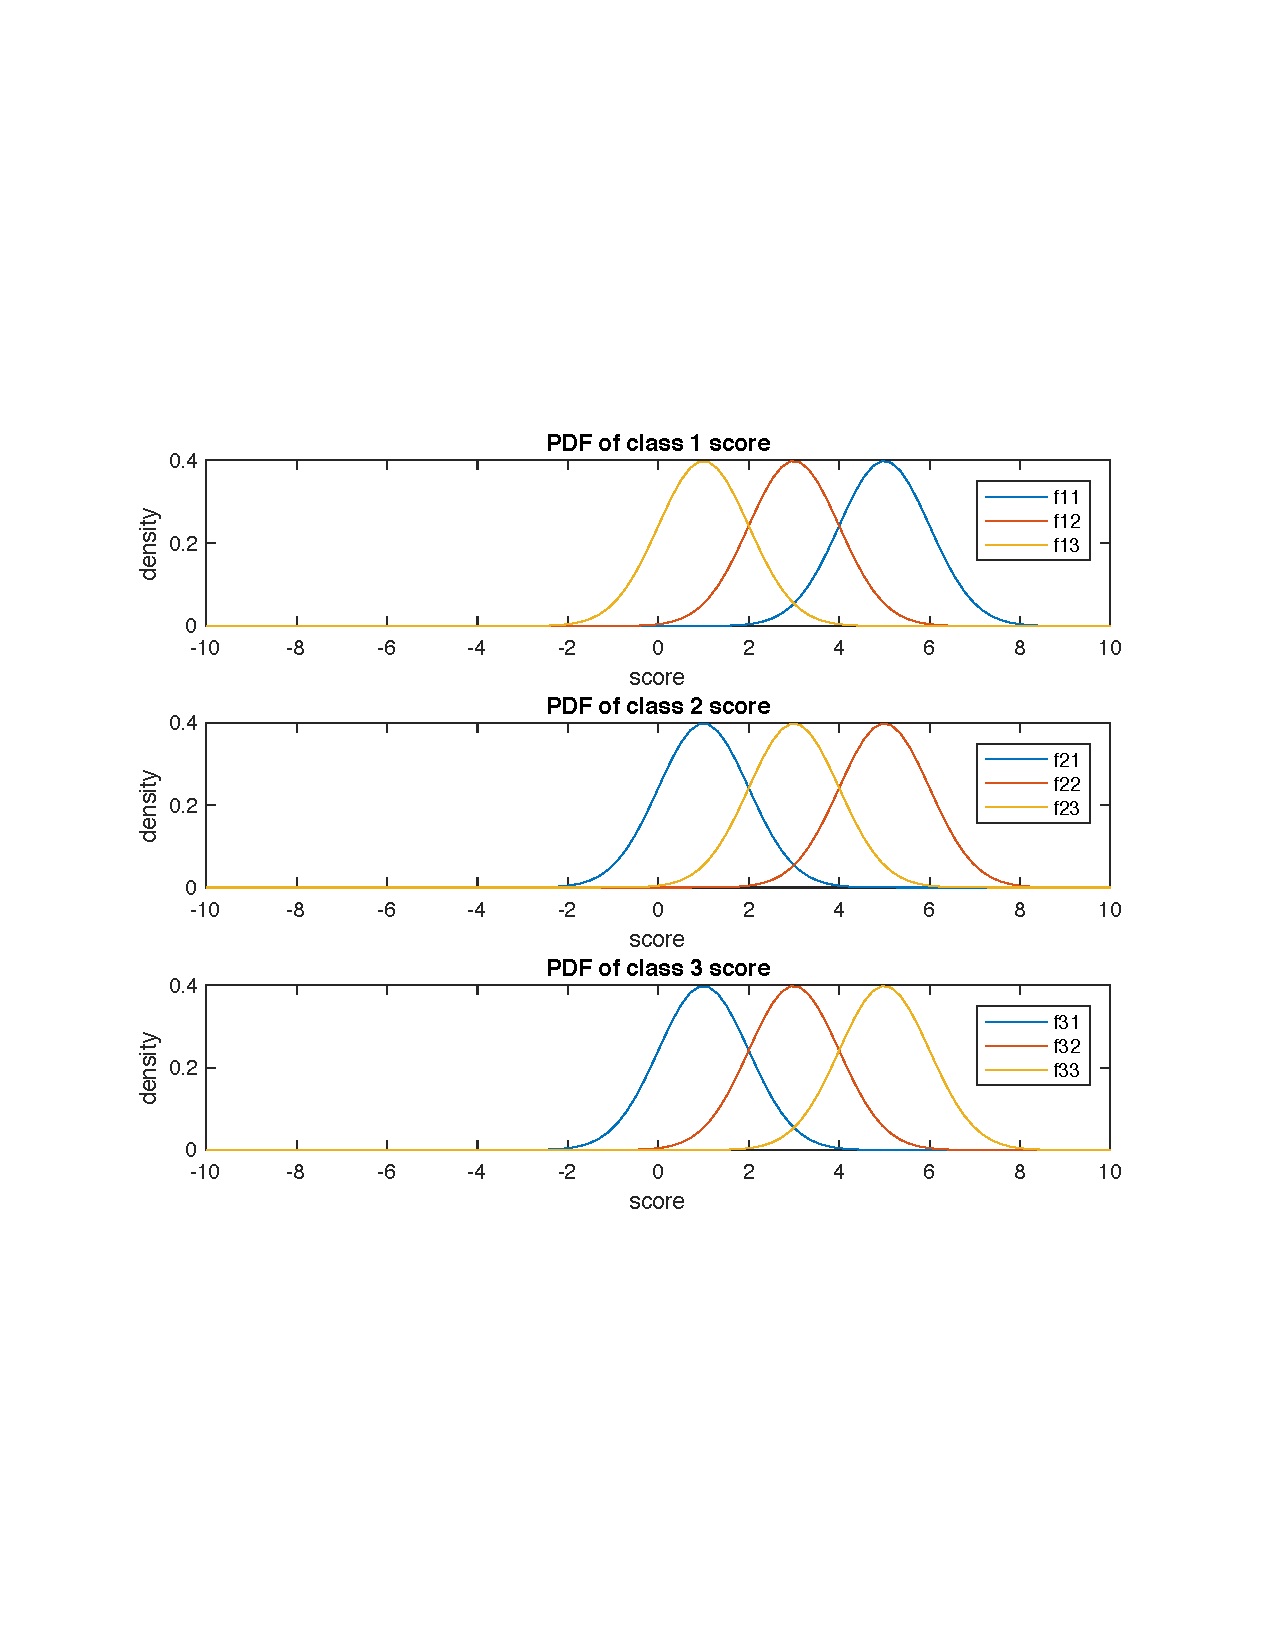
\includegraphics[height=1.9in]{pic/vis_pdf_score_B.pdf}
        \caption{}
    \end{subfigure}%
    ~ 
    \begin{subfigure}[b]{0.5\textwidth}
        \centering
        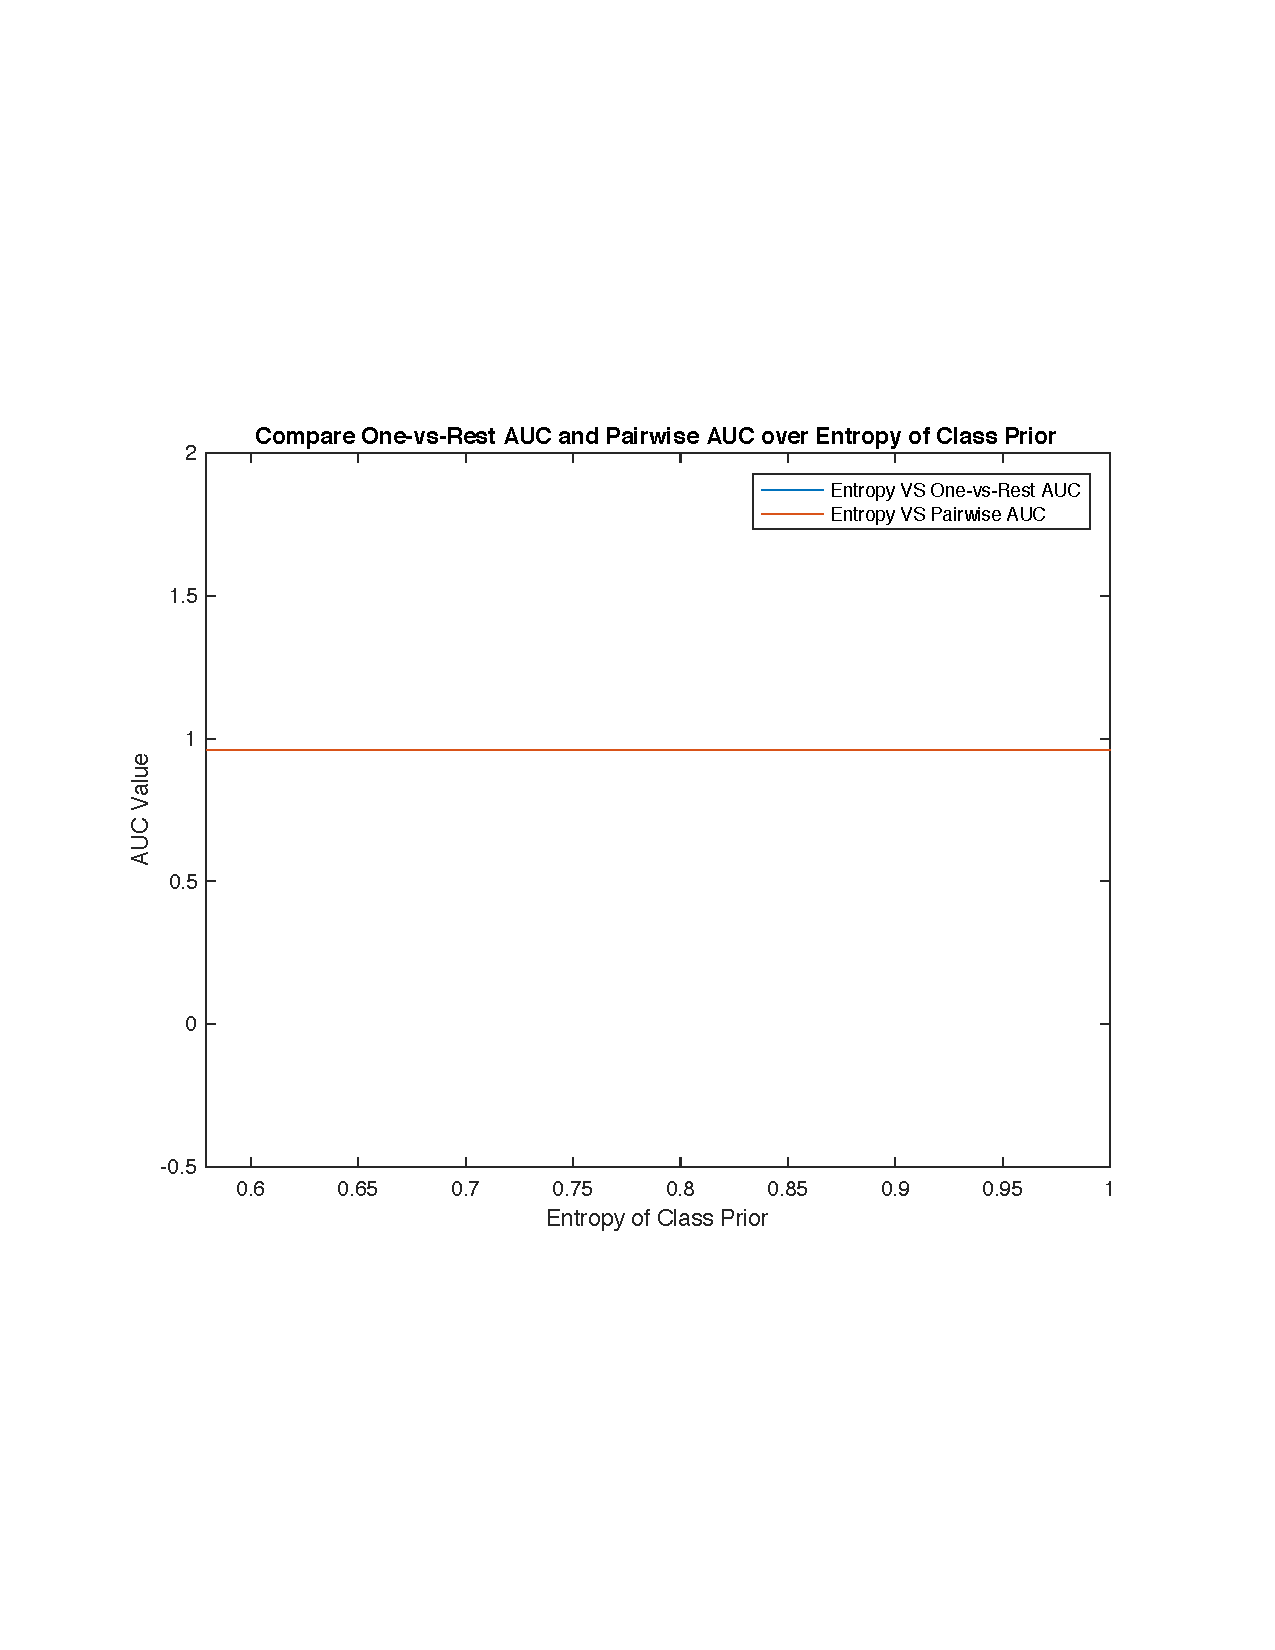
\includegraphics[height=1.9in]{pic/vis_ent_auc_B.pdf}
        \caption{}
    \end{subfigure}
    \caption{One-VS-Rest AUC and Pairwise AUC plotted over the entropy of the probability distribution of the class, with the same separability setting among classes (Situation A).}
    \begin{subfigure}[b]{0.5\textwidth}
        \centering
        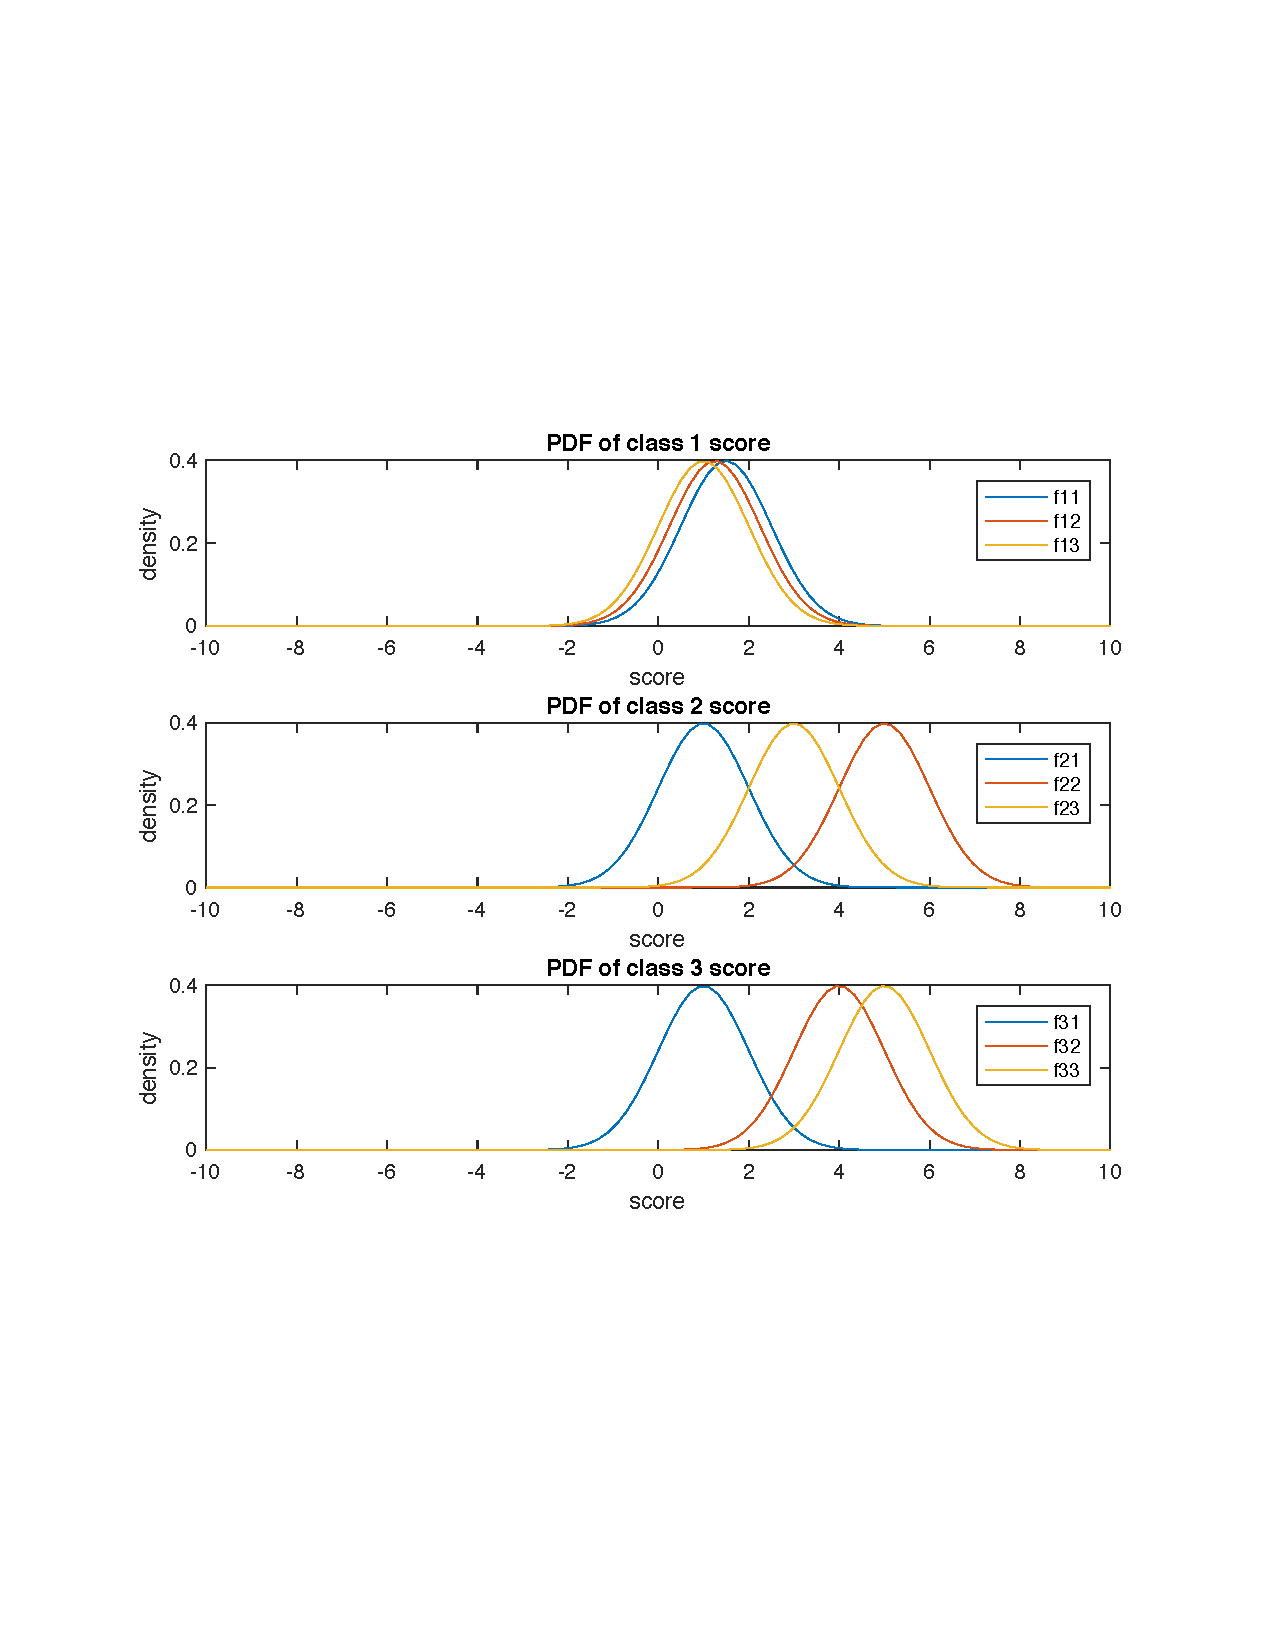
\includegraphics[height=1.9in]{pic/vis_pdf_score_A.pdf}
        \caption{}
    \end{subfigure}%
    ~ 
    \begin{subfigure}[b]{0.5\textwidth}
        \centering
        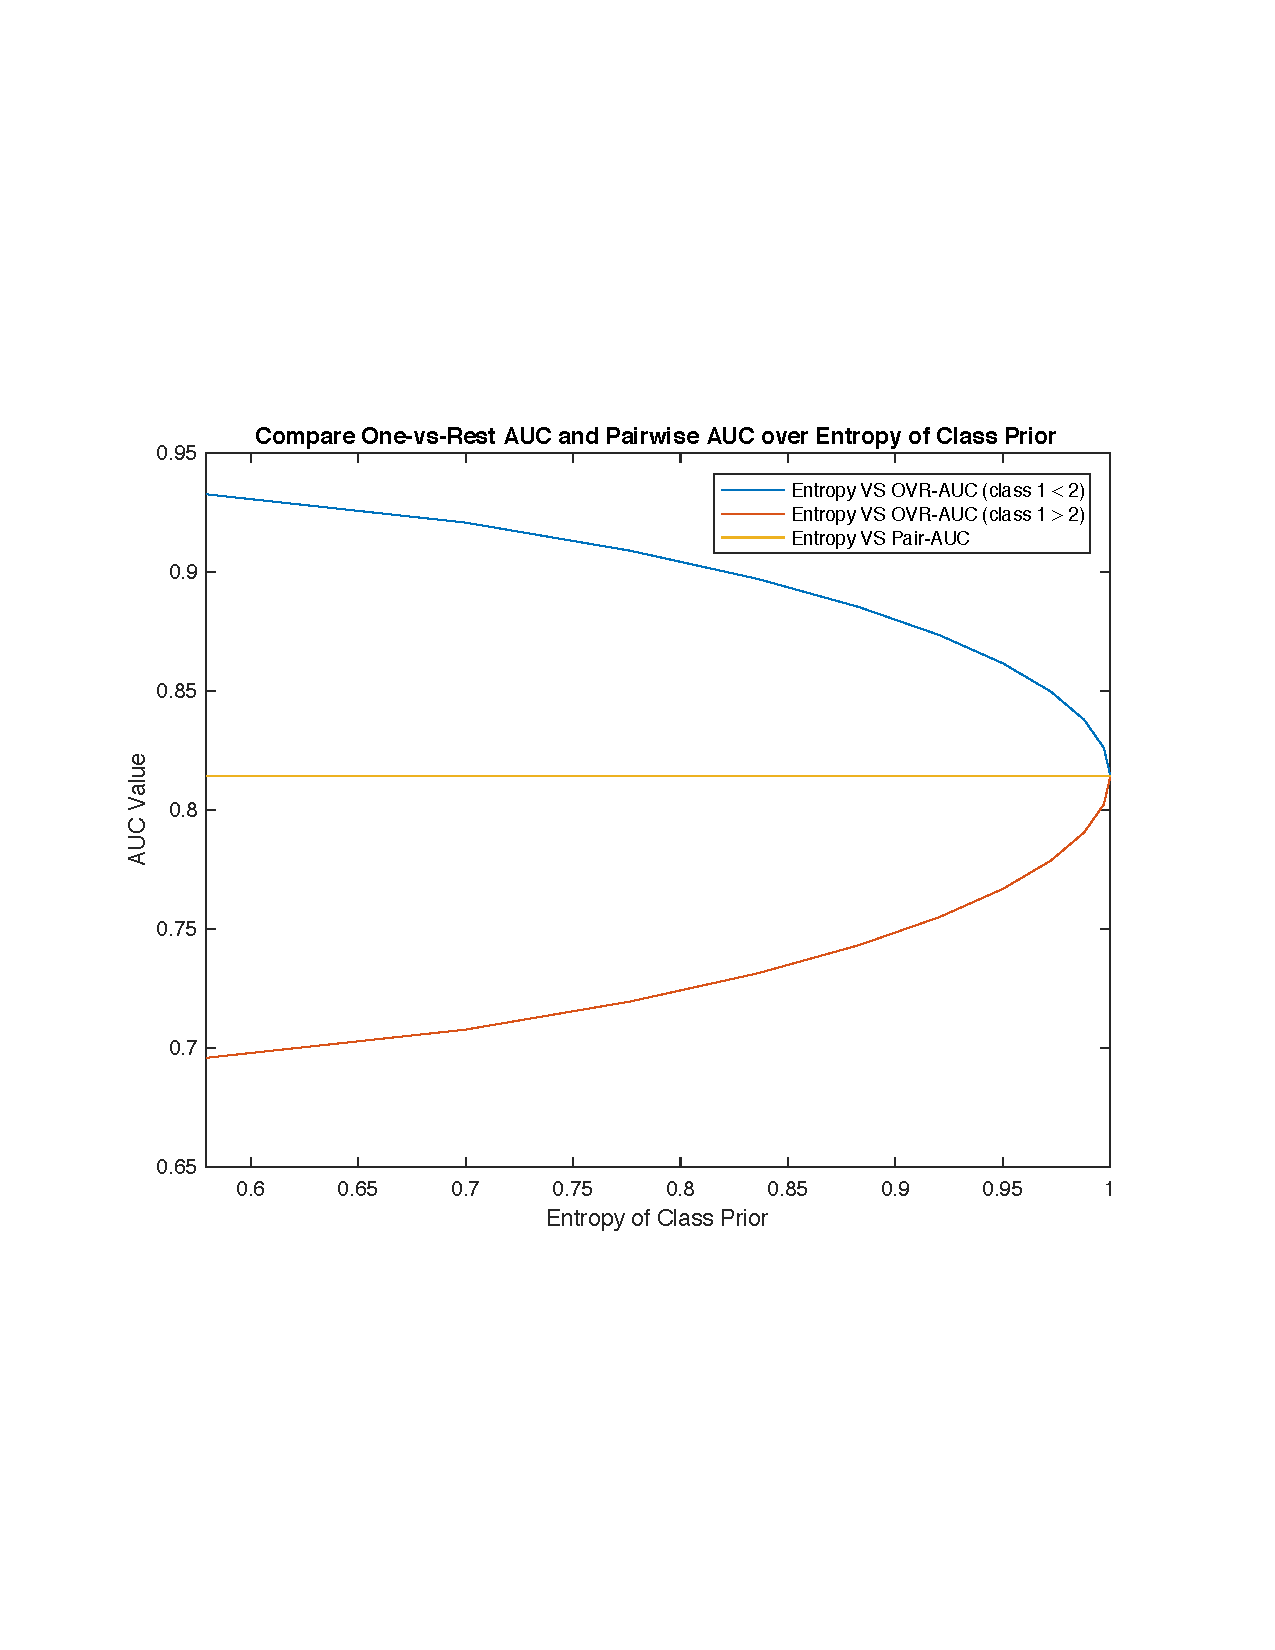
\includegraphics[height=1.9in]{pic/vis_ent_auc_A.pdf}
        \caption{}
    \end{subfigure}
    \caption{One-VS-Rest AUC and Pairwise AUC plotted over the entropy of the probability distribution of the class, with different separability setting among classes (Situation B). }
\end{figure*}

Figure 5 and 6 imply the following:

(1) As the data becomes less imbalanced, one-vs-rest AUC approaches the value of pairwise AUC. 

(2) The value of one-vs-rest AUC can be greater, equal or less than pairwise AUC. When the hard-separable case is more often, such as score axis 3 in Figure 6(a), the one-vs-rest AUC will be lower than pairwise AUC. If the easier-separable case is more prevalent, one-vs-rest AUC will be greater than pairwise AUC.

(3) When all PDFs for each score axis are distributed in the same way, one-vs-rest is insensitive to class imbalance and have the exactly same value as pairwise AUC.

% Based on the experimental results, we find that under the given class separability setting in Situation A, as entropy of the class distribution increases, one-vs-rest AUC increases and becomes equal to pairwise AUC when classes are balanced (entropy is 1). More extent of class imbalance leads to smaller one-vs-rest AUC. AUCs of one-vs-rest are always smaller than AUCs of pairwise in class imbalance settings.

% However, under the score separability setting in Situation B, we find that class imbalance does not affect one-vs-rest AUC values. Pairwise AUC and one-vs-rest AUC have the same value.

%if $f_{ij}$'s are distributed in the same way in each score axis.

%Findings: 1-vs-rest insensitive to class distribution when (positive and res) (res pdfs) distributed in the same way.

\section{Conclusion}
% summarize theoretical and experimental result
% limitation
% future work
\paragraph{Summary:}
We explored the relationships and differences among 3 kinds of multiclass extensions of AUC/ROC (pairwise, one-vs-rest and VUS) theoretically and empirically. We unified binary AUC and the aforementioned extensions using score density function and thresholds. We empirically showed the relationship between pairwise and one-vs-rest AUC and how they are affected by class separability and class imbalance.

\paragraph{Future work:}
One limitation of our work is that the threshold $T_{ij}$ can only be useful when the density function are given. It is necessary to focus on relating such thresholds to actual multiclass classifiers in the future. Successfully relating the thresholds to real classifiers will enable us to derive the correct form of VUS.
% Since in our theoretical derivasion, threshold $T_{ij}$ only appears in AUC formulas, we will consider building the connection between $T_{ij}$ and multiclass classifiers.
What we focused in our experiments is the numerical relationship between pairwise and one-vs-rest AUC. When the number of classes is large, it is also necessary to compare the running time of different multiclass extensions. 

%\section*{Acknowledgments}

\newpage
%============================= BIBLIOGRAPHY ===============================

\bibliographystyle{plain}
\bibliography{references}



\end{document}

%=========================== END DOCUMENT ==============================
